
\subsection{Face Generation from Contours}
\label{sec:contourExp}


\paragraph{Contour Dataset} 
\cxj{Yangbinxin: Add description on the dataset generation.}
%


\paragraph{Photo Generation from Contours}
The Pix2pixHD~\cite{} was applied to the task of translating edges to photos. They successfully generate hiqh-quality photos from contours that are generated from real photos. 
However, when we apply the Pix2pixHD model with hand-drawn sketches which present distinct characteristics from the synthesized contours which are smooth and clean without geometric distortions, it fails to produce good results, as Fig.~\ref{fig:cmp-contour-generation} shows. \cxj{Add more results with other models.}
We can see that \cxj{expected results: (e) have better details. (d) i have no idea.  c is better than (b).} 
%



\begin{figure}
	\centering
	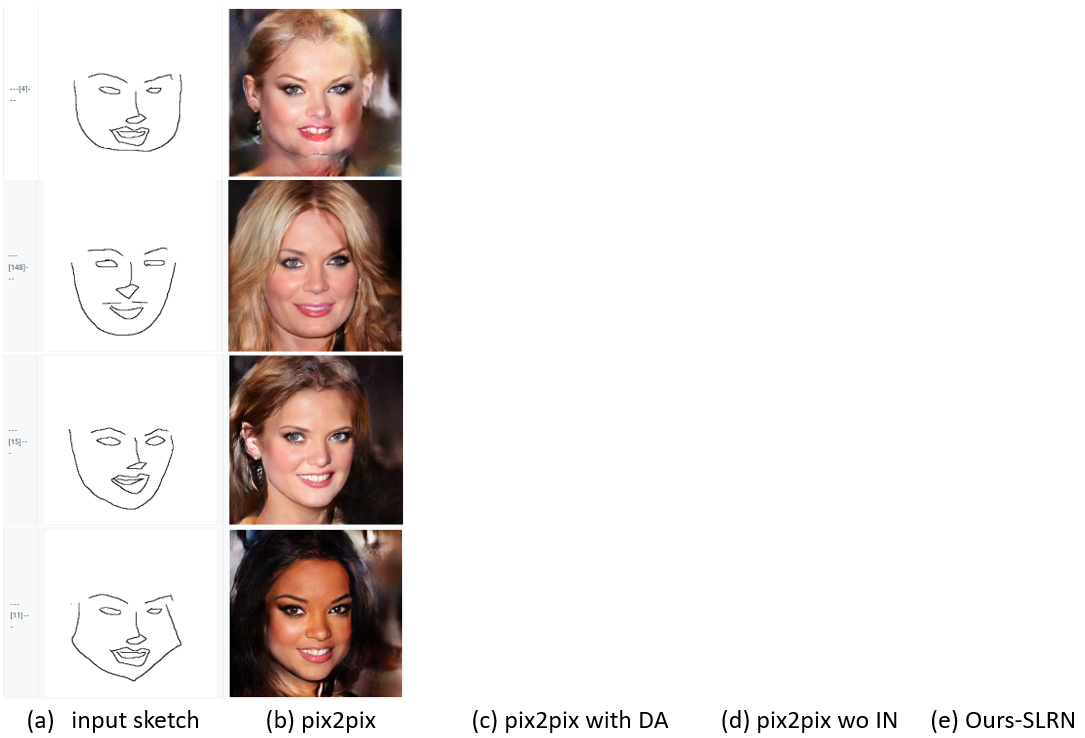
\includegraphics[width=\columnwidth]{figs/contour-generation.png}
	\caption{Face generation with different models. From left to right: (a) hand-drawn sketches as input. (b) Results generated by pix2pixHD that is retrained using our contour-photo dataset. (c) Results generated by pix2pixHD that is retrained using our contour-photo dataset with geometric transformation as data augmentation. (d) Results generated by removing instance normalization at the shallow convolution layers (five layers in the global generator). (e) Results from our model (pix2pixHd architecture by replacing instance normalization with the proposed SLRN. ) More results can be found here: \cxj{Provide a link for all results.}  }
	\label{fig:cmp-contour-generation}
\end{figure}


\paragraph{Face Editing with Strokes} When users want to change local shapes of facial features, a few strokes can be modified in our interface. 
The pix2pixHD model does not take the sparsity of sketches and the instance normalization tends to normalize local regions with a global style factor, which mainly conveys brightness variance. Therefore, when local details such as hair, the bamoustache, and so on, the results change significantly even only local region is modified. 
In comparison, our proposed SLRN captures the shape details in the drawn sketches and successfully avoid edge-aligned artifacts caused by distortion in hand-drawn sketches, as Fig.~\ref{fig:cmp-contour-editing} shows.

\begin{figure}
	\centering
	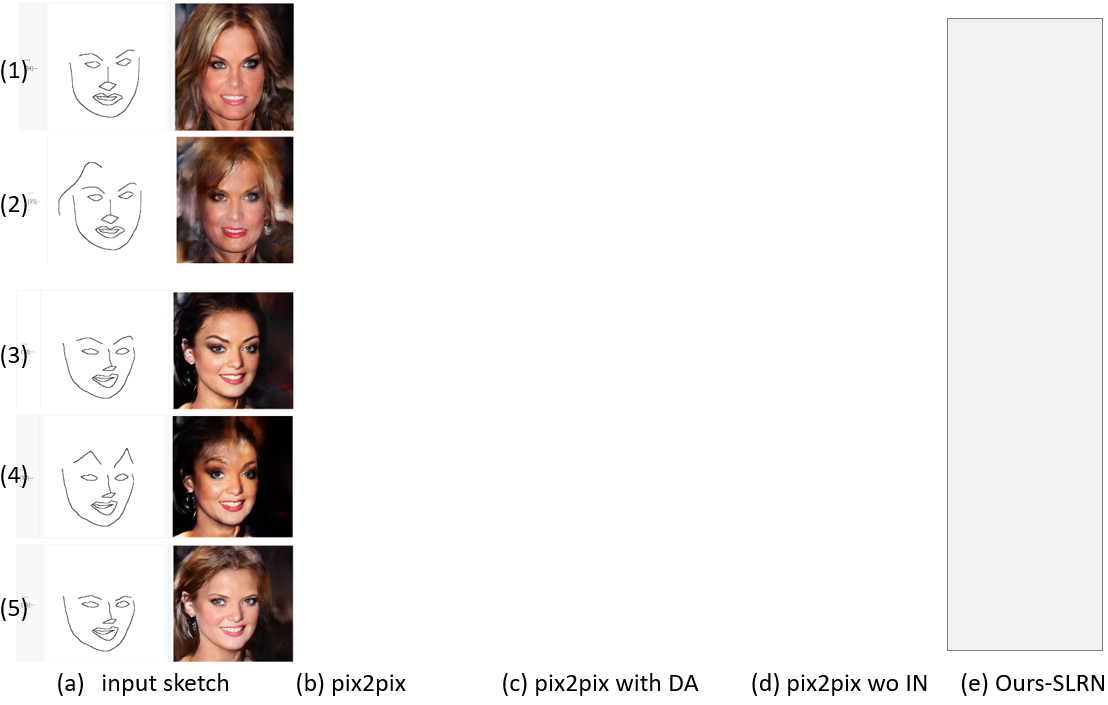
\includegraphics[width=\columnwidth]{figs/contour-editing.png}
	\caption{Local face editing with different models. \td{The proposed SLRN captures the shape details in the drawn sketches and successfully avoid edge-aligned artifacts caused by distortion in hand-drawn sketches.} More results can be found here: \cxj{Provide a link for all results.} }
	\label{fig:cmp-contour-editing}
\end{figure}



\td{In order to analyze the effect of instance normalization and our SLRN, we visualize the features extracted at early stages in the generators of different models.}
As Fig.~\ref{fig:vis-feature-slpn} shows, ....

\begin{figure*} 
	\centering
	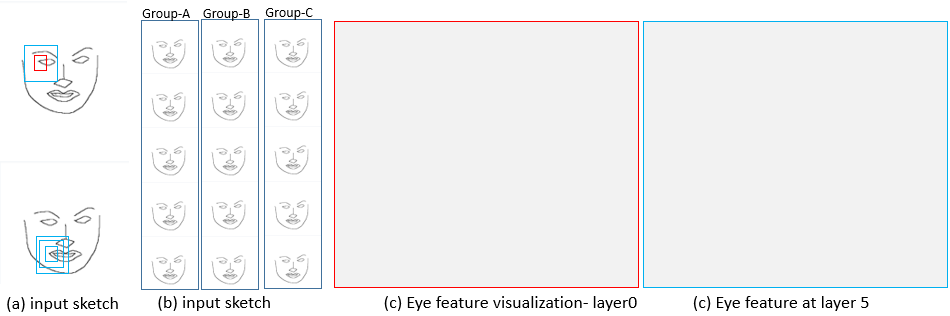
\includegraphics[width=2\columnwidth]{figs/slrnFeature.png}
	\caption{Visualization of extracted features under local editing. We extract the features at different convolution layers at the left eye position (a) from three groups of sketches (b) with different types of local editing. The extracted high-dimensional features using different models including pix2pixHD-DA, pix2pixHD-wo-IN, and our SLRN) are mapped into 2D space using TSNE~\cite{tsne} in (c). \cxj{ChengZhiHua: provide a link for all results.} } 
	\label{fig:vis-feature-slpn}	
\end{figure*}